\documentclass[11pt]{article}
\usepackage[margin=1 in, letterpaper]{geometry}
\usepackage{fontspec, graphicx, amsmath, amssymb, amsthm, array, physics, enumitem, cancel, multicol, float, dsfont}
\usepackage{latexsym, marvosym}
\usepackage[dvipsnames]{xcolor}

\setmainfont{Linux Libertine O}
\setsansfont{Linux Biolinum O}
\setmonofont{Latin Modern Mono}
\setmathrm{Latin Modern Math}
\theoremstyle{definition}
\newtheorem{theo}{\color{Maroon} Theorem}[section] 
\newtheorem{defin}[theo]{\color{Maroon} Definition}
\newtheorem{example}[theo]{\color{Maroon} Example}
\newtheorem{prob}[theo]{\color{Maroon} Problem}
% \newtheorem{example}[section]{\color{Maroon} Example}

\theoremstyle{remark}
\newtheorem*{soln}{\color{Maroon} Solution}

\newcommand{\R}{\mathbb{R}}
\newcommand{\Q}{\mathbb{Q}}
\newcommand{\Z}{\mathbb{Z}}
\newcommand{\N}{\mathbb{N}}
\newcommand{\Bin}{\text{Bin}}
\newcommand{\Bern}{\text{Bern}}

%%%%%%%%%%%%%%%%%%% Statistics %%%%%%%%%%%%%%%%%%%%
\newcommand{\E}[1]{\mathbb{E}\left[ #1 \right]}
\newcommand{\Prob}[1]{\mathbb{P}\left[ #1 \right]}
\newcommand{\cov}{\textnormal{Cov}}
\newcommand{\corr}{\textnormal{Corr}}
\renewcommand{\var}{\textnormal{Var}}
% \newcommand{\cov}[2]{\textnormal{Cov}\left[ #1, #2 \right]}
% \newcommand{\corr}[2]{\textnormal{Corr}\left[ #1, #2 \right]}
% \renewcommand{\var}[1]{\textnormal{Var}\left[ #1 \right]}
\newcommand{\Unif}{\textnormal{Unif}}
\newcommand{\Norm}{\mathcal{N}}
\newcommand{\ind}[1]{\mathds{1}_{#1}} 
\newcommand{\NBin}{\textnormal{NBin}}
\newcommand{\Geom}{\textnormal{Geom}}
\newcommand{\FS}{\textnormal{FS}}
\newcommand{\HGeom}{\textnormal{HGeom}}
\newcommand{\Mult}{\textnormal{Mult}}
\newcommand{\Pois}{\textnormal{Pois}}
\newcommand{\Expo}{\textnormal{Expo}}
\newcommand{\Beta}{\textnormal{Beta}}
\newcommand{\Gam}{\textnormal{Gamma}}
\newcommand\independent{\protect\mathpalette{\protect\independenT}{\perp}}
    \def\independenT#1#2{\mathrel{\setbox0\hbox{$#1#2$}%
    \copy0\kern-\wd0\mkern4mu\box0}} 

%%%%%%%%%%%%%%%%%%%%%%%%%%%%%%%%%%%%%%%%%%%%%%%%%%%%%%%%%%%%%%%%%%%%
\newcommand{\inserttitle}{Section 07}
\newcommand{\insertauthor}{Max Guo \& Seung Hwan An}
\newcommand{\insertcourse}{STAT 110}
%%%%%%%%%%%%%%%%%%%%%%%%%%%%%%%%%%%%%%%%%%%%%%%%%%%%%%%%%%%%%%%%%%%%

\usepackage{fancyhdr}
\setlength{\headheight}{15pt}
\pagestyle{fancy}
\fancyhf{}
\fancyhead[C]{\thepage}
\fancyhead[L]{\inserttitle}
\fancyhead[R]{\insertauthor}

%%%%%%%%%%%%%%%%%%%%%%%%%%%%%%%%%%%%%%%%%%%%%%%%%%%%%%%%%%%%%%%%%%%%

\begin{document}

{\noindent\Huge\bf  \\[0.1\baselineskip] {\inserttitle }}\\[2\baselineskip]
{{\bf \insertcourse}\\ {\textit{November 1, 2021}}} \hfill {\large \textsc{\insertauthor}}
\smallskip

\hfill \noindent \textit{Credits to William Chen and Sebastian Chiu}

\section{Multivariate Random Variables}

Sometimes we have more than one random variable of interest, and we want to study probabilities associated with all of the random variables. Instead of studying the distributions of $X_1, X_2, X_3$ separately, we can study the distribution of the multivariate vector $\textbf{X} = (X_1, X_2, X_3)$. Joint PDFs and CDFs are analogous to multivariate versions of univariate PDFs and CDFs. Usually joint PDFs and PMFs carry more information than the marginal ones do, because they account for the interactions between the various random variables. If, however, the random variables are independent, then the joint PMF/PDF is just the product of the marginals and we get no extra information by studying them jointly rather than marginally.

\subsection{Joint Distributions}
Review: Joint Probability of events $A$ and $B$: $P(A \cap B)$

\begin{table}[h]\begin{center}
	\begin{tabular}{ccccc} \hline
		\textbf{Joint CDF} & ~ & \textbf{Joint PMF} & ~ & \textbf{Joint PDF} \\  \hline
		$F_{X, Y}(x, y) = P(X \leq x,Y \leq y)$ & ~ & $P(X=x, Y=y)$ & ~ & $f_{X,Y}(x,y) = \frac{\delta}{\delta x} \frac{\delta}{\delta y}F_{X, Y}(x, y)$ \\  \hline
	\end{tabular}\end{center}
\end{table}

Both the Joint PMF and Joint PDF must be non-negative and sum/integrate to 1. $$\sum_x \sum_y P(X=x, Y=y) = 1 \text{ (discrete)} \quad \int_x\int_y f_{X,Y}(x,y) = 1 \text{ (continuous)}$$ Like in the univariate cause, you sum/integrate the PMF/PDF to get the CDF.

\subsection{Conditional Distributions}
Review: By Bayes' Rule, $P(A|B) = \frac{P(B|A)P(A)}{P(B)}$ Similar conditions apply to conditional distributions of random variables.\\

For discrete random variables:
\[P(Y=y|X=x) = \frac{P(X=x, Y=y)}{P(X=x)} = \frac{P(X=x|Y=y)P(Y=y)}{P(X=x)}\]
For continuous random variables:
\[f_{Y|X}(y|x) = \frac{f_{X,Y}(x, y)}{f_X(x)} = \frac{f_{X|Y}(x|y)f_Y(y)}{f_X(x)}\]
Hybrid Bayes' Rule (for event $A$ and random variable $X$)
\[f_X(x|A) = \frac{P(A | X = x)f_X(x)}{P(A)}\]


\subsection{Marginal Distributions}
Review: Law of Total Probability Says for an event $A$ and partition $B_1, B_2, ... B_n$: $P(A) = \sum_i P(A\cap B_i)$ \\ \\
To find the distribution of one (or more) random variables from a joint distribution, sum or integrate over the other random variables. \\

\noindent
Getting the Marginal PMF from the Joint PMF
\[P(X = x) = \sum_y P(X=x, Y=y)\]
Getting the Marginal PDF from the Joint PDF
\[f_X(x) = \int_y f_{X, Y}(x, y) dy\]


\subsection{Multivariate LOTUS}
Review: $E(g(X)) = \sum_xg(x)P(X=x)$, or $E(g(X)) = \int_{-\infty}^{\infty}g(x)f_X(x)dx$\\ \\ 
For discrete random variables:
\[E(g(X, Y)) = \sum_x\sum_yg(x, y)P(X=x, Y=y)\]
For continuous random variables:
\[E(g(X, Y)) = \int_{-\infty}^{\infty}\int_{-\infty}^{\infty}g(x, y)f_{X,Y}(x, y)dxdy\]
This is because a joint random variable \textit{is} a random variable. You can imagine that instead of there being a pair of random variables $X$ and $Y$, that there is a single random variable $(X,Y)$ with distribution $f_{X,Y}(x,y)$. 

\subsection{Independence of Random Variables}
Review: $A$ and $B$ are independent if and only if either $P(A\cap B) = P(A)P(B)$ or $P(A|B) = P(A)$. \\

Similar conditions apply to determine whether random variables are independent - two random variables are independent if their joint distribution function is simply the product of their marginal distributions, or that the a conditional distribution of is the same as its marginal distribution. \\

In words, random variables $X$ and $Y$ are independent for all $x, y$, if and only if one of the following hold:
\begin{itemize}
	\itemsep -1mm
	\item Joint PMF/PDF/CDFs are the product of the Marginal PMF
	\item Conditional distribution of $X$ given $Y$ is the same as the marginal distribution of $X$
\end{itemize}

\begin{table}[htb]
	\begin{tabular}{ccc}
		X and Y (discrete) are independent  & $\Longleftrightarrow$ & $P(X \leq x, Y \leq y) = P(X \leq x)P(Y \leq y),  \forall x, y$ \\ 
		X and Y (discrete) are independent  & $\Longleftrightarrow$ & $P(X=x, Y=y) = P(X=x)P(Y=y),  \forall x, y$ \\ 
		X and Y (discrete) are independent  & $\Longleftrightarrow$ & $P(X=x | Y=y) = P(X=x),  \forall x, y$ \\ 
		X and Y (continuous) are independent  & $\Longleftrightarrow$ & $P(X \leq x, Y \leq y) = P(X \leq x)P(Y \leq y),  \forall x, y$ \\ 
		X and Y (continuous) are independent  & $\Longleftrightarrow$ & $f_{X, Y}(x, y) = f_X(x)f_Y(y), \forall x, y$ \\ 
		X and Y (continuous) are independent  & $\Longleftrightarrow$ & $f_{X|Y}(X|Y) = f_X(X), \forall x, y$ 
	\end{tabular}
\end{table}



\section{Covariance and Correlation}
\begin{figure}[H]\centering
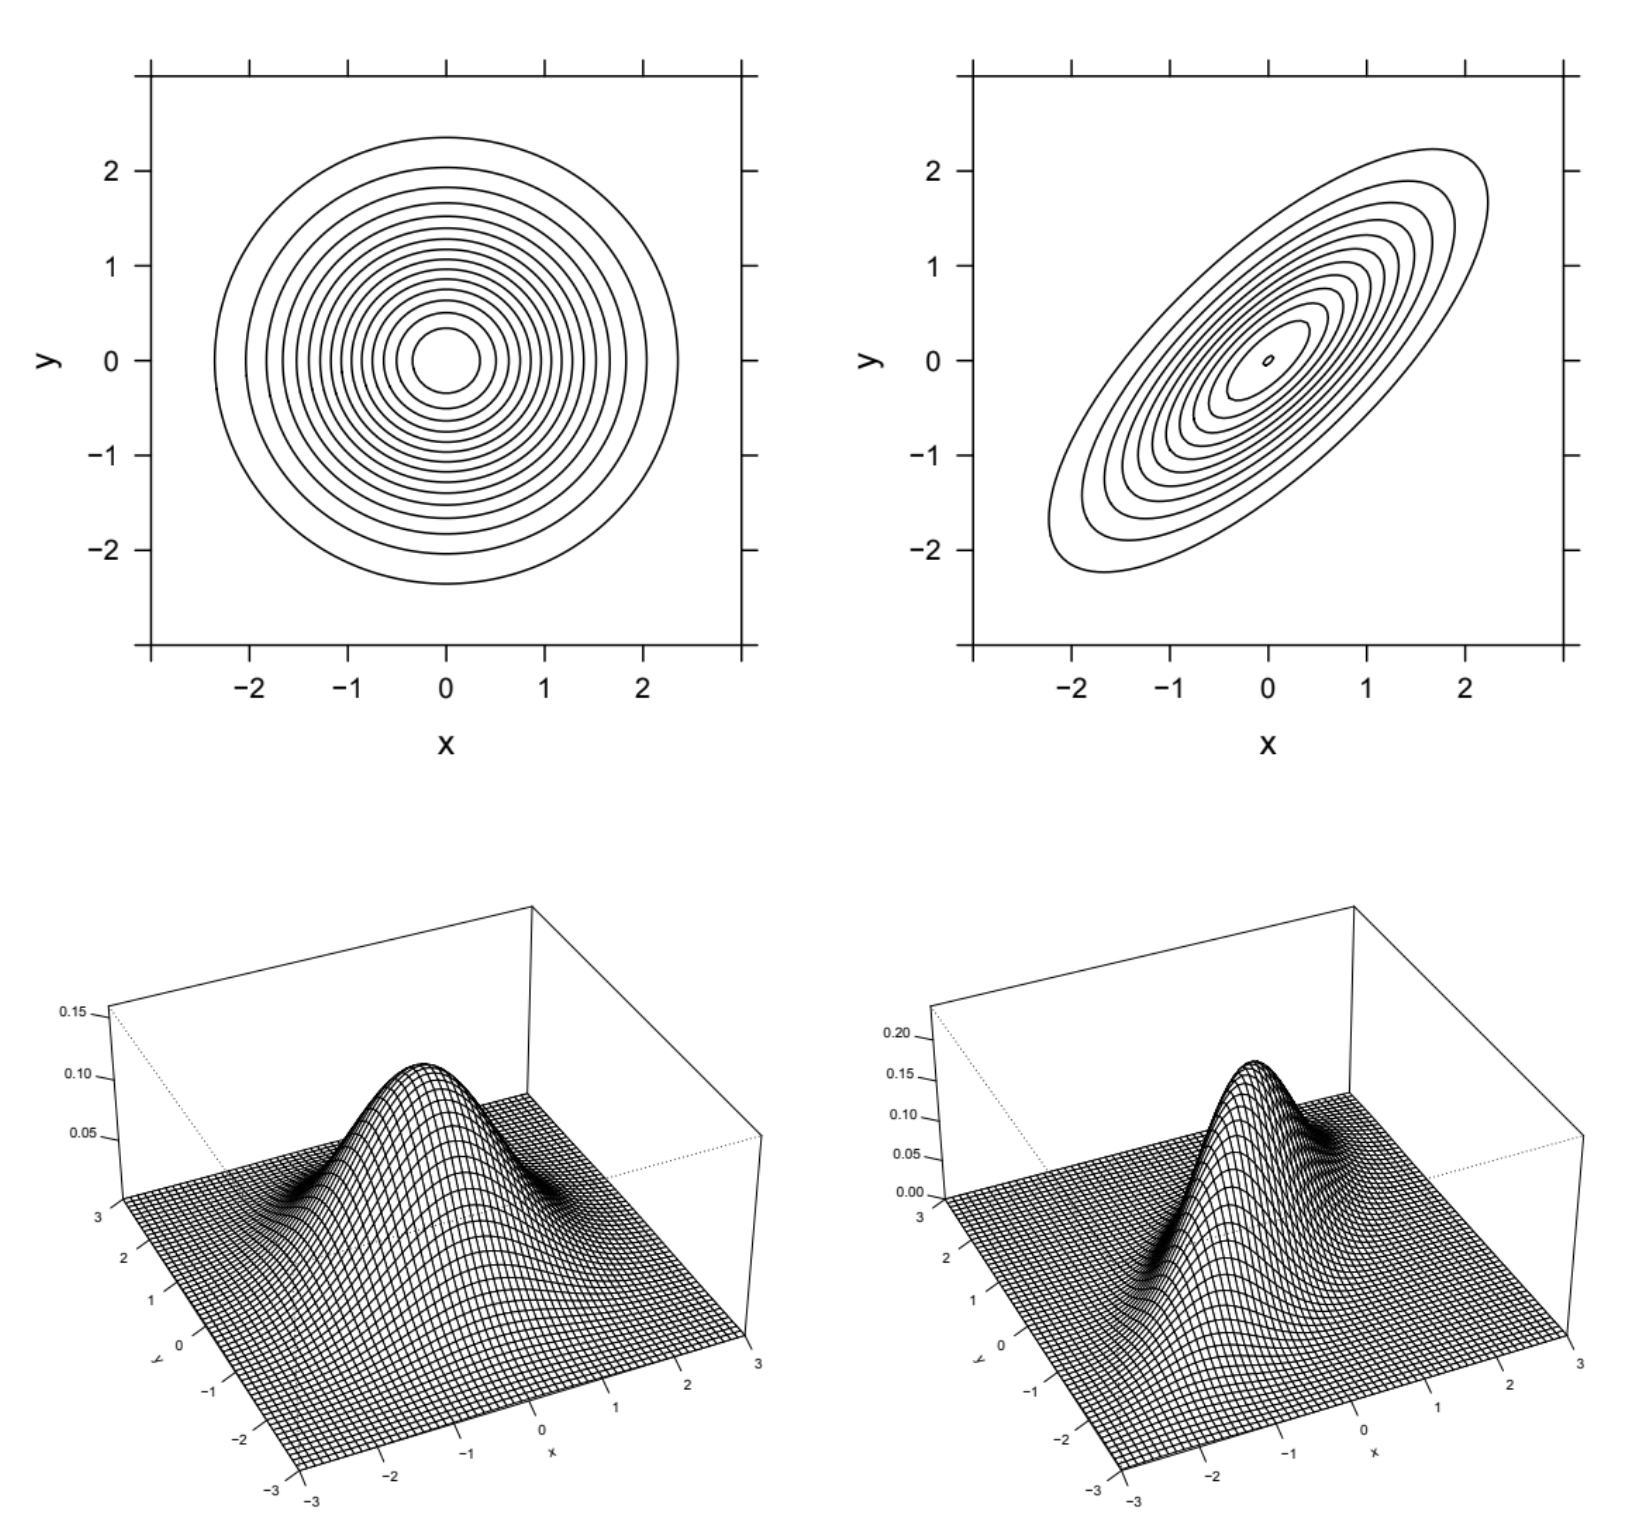
\includegraphics[width = 0.9\textwidth]{image/BVN.png}
\caption{(left) We have two uncorrelated distributions that are marginally identical. (right) We have two positively correlated distributions that are marginally identical. If we know that one of them is high relative to the mean, then we know that the the other one is likely to be high relative to the mean too. Plots courtesy of Jessy Hwang.}
\end{figure}

\begin{description}
\item [Covariance] is the two-random-variable equivalent of Variance, defined by the following:
	\[\cov(X, Y) = E[(X - E(X))(Y - E(Y))] = E(XY) - E(X)E(Y)\]
	Note that 
	\[\cov(X, X) = E(XX) - E(X)E(X) =  E(X^2) - [E(X)]^2 = \var(X)\]
\item [Correlation] is a rescaled variant of Covariance that is always between -1 and 1.
	\[\corr(X, Y) = \frac{\cov(X, Y)}{\sqrt{\var(X)\var(Y)}} = \frac{\cov(X, Y)}{\sigma_X\sigma_Y}\]
\item [Covariance and Indepedence] - If two random variables are independent, then they are uncorrelated. The inverse is not necessarily true. 
	\[X \independent Y \longrightarrow \cov(X, Y) = 0\]

\begin{example} Can you think of the case where $\cov(X_1,X_2)=0$ but $X_1$ and $X_2$ are dependent?

\vspace{1 in}

% Consider $X_1 = Y_1 + Y_2$ and $X_2 = Y_1 - Y_2$, where $Y_1,Y_2 \overset{\text{iid}}{\sim} \Bern(1/2)$. Then, using the properties below, $$ \cov(X_1,X_2) = \var(Y_1) - \var(Y_2) = 0 $$ But knowing $X_1$ does give information about $X_2$, since if $X_1 = 2$, it tells us that $Y_1,Y_2=1$, and thus $X_2 = 0$. 

\end{example}

%, except in the case of Multivariate Normal, where uncorrelated \emph{does} imply independence.
\item [Covariance and Variance] - Note that
	\begin{align*}
		\cov(X, X) &= \var(X) \\
		\var(X + Y) &= \var(X) + \var(Y) + 2\cov(X, Y) \\
		\var(X_1 + X_2 + \dots + X_n ) &= \sum_{i = 1}^{n}\var(X_i) + 2\sum_{i < j} \cov(X_i, X_j)
	\end{align*}
	In particular, if X and Y are independent then they have covariance 0 thus
	\[X \independent Y \Longrightarrow \var(X + Y) = \var(X) + \var(Y)\]
	In particular, If $X_1, X_2, \dots, X_n$ are i.i.d. and all of them have the same covariance relationship, then 
	\[\var(X_1 + X_2 + \dots + X_n ) = n\var(X_1) + 2{n \choose 2}\cov(X_1, X_2)\]
	
\item [Covariance and Bilinearity] - For random variables $W, X, Y, Z$ and constants $a, b, c, d$:
	\begin{align*}
		\cov(X + b, Y + c) &= \cov(X, Y) \\
		\cov(aX, dY) &= ad\cov(X, Y) \\
		\cov(W + X, Y + Z) &= \cov(W, Y) + \cov(W, Z) + \cov(X, Y) + \cov(X, Z)
	\end{align*}
\item [Covariance and Invariance] - Correlation, Covariance, and Variance are addition-invariant, which means that adding a constant to the term(s) does not change the value. Let $b$ and $c$ be constants.
	\begin{align*}
		\var(X + c) &= \var(X) \\
		\cov(X + b, Y + c) &= \cov(X, Y) \\
		\corr(X + b, Y + c) &= \corr(X, Y) 
	\end{align*}
	In addition to addition-invariance, Correlation is \emph{scale-invariant}, which means that multiplying the terms by any constant does not affect the value. Covariance and Variance are not scale-invariant.
	\[\corr(2X, 3Y) = \frac{\cov(2X, 3Y)}{\sqrt{\var(2X)\var(3Y)}} = \frac{6\cov(X, Y)}{\sqrt{36\var(X)\var(Y)}} = \frac{\cov(X, Y)}{\sqrt{\var(X)\var(Y)}} = \corr(X, Y)\]
\end{description}


\section{Distribution Chart}

\section*{Discrete Distributions}
\begin{center}
\renewcommand{\arraystretch}{3}
\begin{tabular}{cccccc}
\textbf{Distribution} & \textbf{PDF and Support} & \textbf{EV}  & \textbf{Var} & \textbf{MGF}\\
\hline
\shortstack{Bernoulli \\ \Bern($p$)} & \shortstack{$P(X=1) = p$ \\$ P(X=0) = q$} & $p$ & $pq$ & $q + pe^t$ \\
\hline
\shortstack{Binomial \\ \Bin($n, p$)} & \shortstack{$P(X=k) = {n \choose k}p^k(1-p)^{n-k}$  \\ $k \in \{0, 1, 2, \dots n\}$}& $np$ & $npq$ & $(q + pe^t)^n$ \\
\hline
\shortstack{Geometric \\ \Geom($p$)} & \shortstack{$P(X=k) = q^kp$  \\ $k \in \{$0, 1, 2, \dots $\}$}& $\frac{q}{p}$ & $\frac{q}{p^2}$ & $\frac{p}{1-qe^t}, qe^t < 1$\\
\hline
\shortstack{Negative Binomial \\ \NBin($r, p$)} & \shortstack{$P(X=n) = {n+r - 1 \choose r -1}p^rq^n$ \\ $n \in \{$0, 1, 2, \dots $\}$} & $r\frac{q}{p}$ & $r\frac{q}{p^2}$ &  $(\frac{p}{1-qe^t})^r, qe^t < 1$\\
\hline
\shortstack{Hypergeometric \\ \HGeom($w, b, n$)} & \shortstack{$P(X=k) = \frac{{w \choose k}{b \choose n-k}}{{w + b \choose n}}$ \\ $k \in \{$0, 1, 2, \dots $\}$} & $n\frac{w}{b+w}$ & &   \\
\hline
\shortstack{Poisson \\ \Pois($\lambda$)} & \shortstack{$P(X=k) = \frac{e^{-\lambda}\lambda^k}{k!}$ \\ $k \in \{$0, 1, 2, \dots $\}$} & $\lambda$ & $\lambda$ & $e^{\lambda(e^t-1)}$ \\
\hline
\shortstack{Multinomial \\ \Mult$_k(n, \vec{p}$)} & \shortstack{$P(\vec{X} = \vec{n}) = {n \choose n_1n_2\dots n_k}p_1^{n_1}\dots p_k^{n_k}$ \\ $n = n_1 + n_2 + \dots + n_k$} & $n\vec{p}$ & &  \\

\end{tabular}
\end{center}


\section*{Continuous Distributions}
\begin{center}
\renewcommand{\arraystretch}{3}
\begin{tabular}{cccccc}
\textbf{Distribution} & \textbf{PDF and Support} & \textbf{EV}  & \textbf{Var}  & \textbf{MGF}\\
\hline

\shortstack{Uniform \\ \Unif($a, b$)} & \shortstack{$ f(x) = \frac{1}{b-a}, x \in [a, b] $ \\$ f(x) = 0, x \notin [a, b]$} & $\frac{a+b}{2}$ & $\frac{(b-a)^2}{12}$ &  $\frac{e^{tb}-e^{ta}}{t(b-a)}$\\
\hline
\shortstack{Normal \\ $\N(\mu, \sigma^2)$} & \shortstack{$f(x) = \frac{1}{\sigma \sqrt{2\pi}} e^{-\frac{(x - \mu)^2}{2 \sigma^2}}$ \\ $x \in (-\infty, \infty)$} & $\mu$  & $\sigma^2$ & $e^{t\mu + \frac{\sigma^2t^2}{2}}$\\
\hline
\shortstack{Exponential \\ $\Expo(\lambda)$} & \shortstack{$f(x) = \lambda e^{-\lambda y}, x \in [0, \infty)$\\$ f(x) = 0, x \notin [0, \infty)$} & $\frac{1}{\lambda}$  & $\frac{1}{\lambda^2}$ & $\frac{\lambda}{\lambda - t}, t < \lambda$\\
\hline
\shortstack{Multivariate Uniform \\ A is area of support} & \shortstack{$f(x) = \frac{1}{A}, x \in A$\\$ f(x) = 0, x \notin A $} & $$  & ~ & $$\\
\hline

\end{tabular}
\end{center}

\section*{Practice Problems}
% \vskip .2 in

\begin{prob}{\bf Probabilities Using Joint CDFs and PDFs.} Let $X$ and $Y$ be continuous random variables. What is the probability that $(X,Y)$ falls into the 2-D rectangle $[a_1, a_2] \times [b_1, b_2]$ in terms of a) The joint CDF of $X$ and $Y, F(x,y),$ and b) The joint PDF of $X$ and $Y, f(x,y)$?
\end{prob}

\fbox{\parbox{0.9 \textwidth}{
The joint CDF $F(x,y) = P(X \le x, Y \le y)$. Thus we have:
\begin{align*}
    P( a_1 \le X \le a_2, b_1 \le Y \le b_2) &= P(X \le a_2, Y \le b_2) - P(X \le a_1, Y \le b_2) \\ &- P(X \le a_2, Y \le b_1) + P(X \le a_1, Y \le b_1) \\
    &= F(a_2, b_2) - F(a_1, b_2) - F(a_2, b_1) + F(a_1, b_1)
\end{align*}
The desired probability can be represented in terms of the joint PDF as:
\begin{align*}
    P( a_1 \le X \le a_2, b_1 \le Y \le b_2) &= \int_{b_1}^{b_2} \int_{a_1}^{a_2} f(x, y) \mathrm dx \mathrm dy
\end{align*}
}}

\vskip 2in

\begin{prob}{\bf Stick Breaking. } Suppose a stick of length 1 is randomly broken into three pieces. Find the probability that no piece is longer than 2/3.
\end{prob}

\fbox{\parbox{0.9 \textwidth}{
Let $X, Y$ be independent and distributed $\Unif[0,1]$. We first look at the case where $X < Y$. Then the lengths of the three pieces are $X$, $Y - X$, and $1 - Y$. If no piece is longer than $2/3$, then $X \le 2/3$, $Y > 1/3$, and $X \le Y \le X + 2/3$. \\

Since $(X, Y)$ is Uniform over the square where $0 \le x \le 1$ and $0 \le y \le 1$, the probability of a subregion is proportional to its area. Looking only at the region where $X < Y$, the region where $x \le 2/3$, $y > 1/3$, and $x \le y \le x + 2/3$ has area $1/3$.\\

Looking only at the region where $Y < X$, the corresponding area is also $1/3$ by symmetry. Therefore, the probability that no piece is longer than $2/3$ is $1/3 + 1/3 = 2/3$.

\begin{center}
    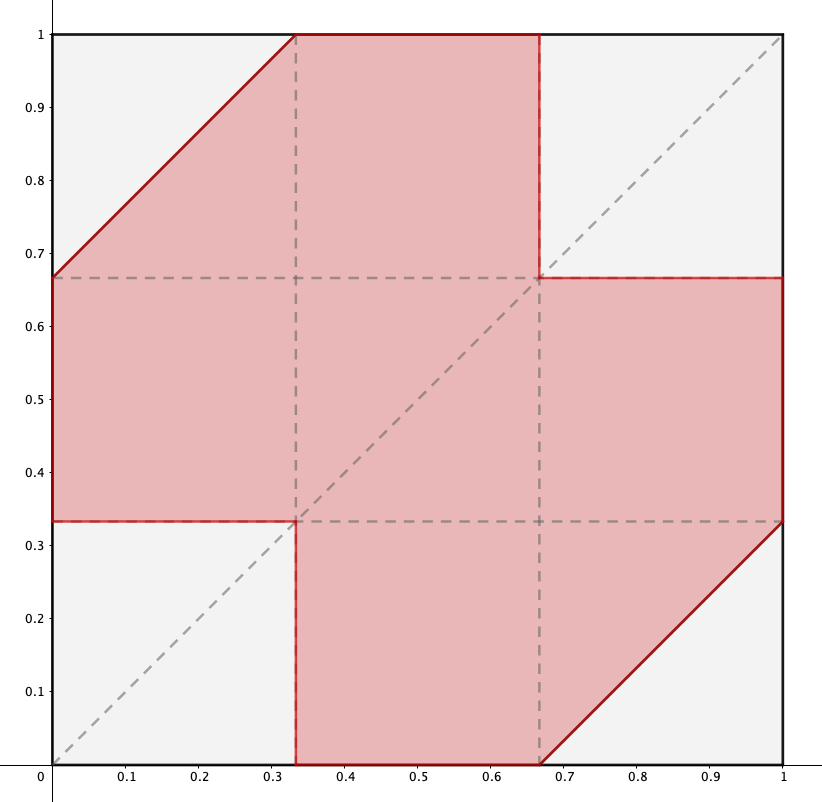
\includegraphics[width=0.5\textwidth]{image/uniformsquare.png}
\end{center}
}}

% \vskip 2.6in

\pagebreak

\begin{prob}{\bf Working with a Joint PDF} \ \ The joint density function of $X$ and $Y$ is $f(x,y) = x+y$, where $0<x<1$ and $0<y<1$.
\begin{enumerate}
         \item Are $X$ and $Y$ independent?
  
\vspace{ 2 in }  
         
\fbox{\parbox{0.9 \textwidth}{
Note that if two continuous random variables are independent, their joint PDF must be the product of their marginal PDFs. So, we can chek if $f(x,y) = f_X(x)f_Y(y)$.\\

Here, we can find the marginal PDF of $X$. By symmetry, the marginal PDF of $Y$ takes the exact same form. The marginal PDF of $X$ is:
\begin{align*}
    f_X(x) = \int_{0}^1 (x+y)\mathrm dy = x + \frac{1}{2}
\end{align*}
Note that $f(x,y) \neq f_X(x)f_Y(y)$ because $x + y \neq (x+1/2)(y+1/2)$, so $X$ and $Y$ are not independent.
}}

         \item Find $P(X+Y>3/2)$ 
         
\vspace{ 2 in }
         
\fbox{\parbox{0.9 \textwidth}{
To calculate this probability, note that $X$ must be at least $1/2$ (because $Y$ can't be greater than $1$, so if $X$ is less than $1/2$ the sum cannot be greater than $3/2$). Consequently, we want to find the probability that $Y$ is greater than $3/2 - X$ under the constraint that $Y < 1$. It follows then that \begin{align*}
    P(X + Y > 3/2) &= \int_{1/2}^1 \int_{3/2 - x}^1 (x + y) dydx \\
    &= \int_{1/2}^1 \left( x- \frac 1 2\right)\left( \frac 5 4 + \frac 1 2 x\right) dx \\
    &= \frac5 {24}.
\end{align*}
}}

	\item Find the conditional density $f(x|y)$.

\vspace{1 in}
	
\fbox{\parbox{0.9 \textwidth}{
From the definition of conditional density (another application of Bayes' Rule!), we know that:
\begin{align*}
    f_{X | Y} (x | y) &= \frac{f_{X,Y}(x,y)}{f_Y(y)} = \frac{x+y}{y + 1/2}
\end{align*}
}}

	\item Set up an integral to determine the expected value $E(XY)$.
	
\fbox{\parbox{0.9 \textwidth}{
Using the 2D LOTUS learned in class, we find that:
\[
E[XY] = \int_0^1 \int_0^1 xy(x+y)dydx = \frac{1}{3}
\]
}}
	
\end{enumerate}
\end{prob}

\pagebreak

\begin{prob}{\bf Correlation and Covariance. }(BH 7.41)\ \ Let $X$ and $Y$ be standardized r.v.s (marginally they each have mean 0 and variance 1) with correlation $\rho \in (-1, 1)$. Find $c,d$ (in terms of $\rho$) such that $Z = X $ and $W = cX + dY$ are uncorrelated but still standardized.
\end{prob}

\fbox{\parbox{0.9 \textwidth}{
Note that, because $X$ and $Y$ are standardized, we have:
\begin{align*}
    \var(X) &= 1 = E[X^2] - E[X]^2 = E[X^2] - 0 \implies E[X^2] = 1 \\
    \var(Y) &= 1 = E[Y^2] - E[Y]^2 = E[Y^2] - 0 \implies E[Y^2] = 1 \\
    \corr(X,Y) &= \rho = \frac{E[XY] - E[X]E[Y]}{\sqrt{\var(X)\var(Y)}} = E[XY]
\end{align*}
We also have $E[Z] = E[W] = 0$ (by linearity), so $X$ and $W$ being uncorrelated is equivalent to $E[WZ] = 0$:
\begin{align*}
    E[WZ] &= E[(cX + dY)X] = cE[X^2] + dE[XY] \\
    &= c + d\rho
\end{align*}
which implies we must have $c = -d\rho$. Furthermore, we must require $\var(W) = 1$:
\begin{align*}
    \var(cX + dY) &= c^2 \var(X) + d^2 \var(Y) + 2\cov(cX, dY) \\
    &= c^2 + d^2 + 2cd\cov(X, Y) \\
    &= c^2 + d^2 + 2cd\corr(X,Y) \quad \text{because $X$, $Y$ are standardized}\\
    &= c^2 + d^2 + 2cd\rho \\
    &= d^2 (1 + \rho^2) - 2\rho^2 d^2 \\
    &= d^2(1 - \rho^2) \\
    &= 1
\end{align*}
Substituting $c = -d\rho$ and solving, we obtain that $d = \frac{1}{\sqrt{1 - \rho^2}}$ and $c = \frac{-\rho}{\sqrt{1 - \rho^2}}$.
}}

\end{document}